%----- do not modify this first block,

\documentclass[sigconf, nonacm, preprint]{acmart}
\usepackage{tabularx}
\usepackage{natbib}
\usepackage{hyperref}
\usepackage{subfig}
\usepackage{graphicx}
\usepackage{enumitem}
\usepackage{xcolor}
\usepackage{multirow}
\usepackage[none]{hyphenat}


\begin{document}
\title{Which performance indicator is meaningful?}
\author{Candidate Number 074936}

\emergencystretch 5em
%% Short summary of the report
\begin{abstract}
	The use of Evolutionary Algorithms (EA) have been popular in solving different types of multi-objective problems (MOP), particularly due to their advantages over classical and gradient-based algorithms. How effective EA are towards different problems, and how we measure their efficiency form the basis of this study. The measures used to quantify effectiveness of multi-objective Evolutionary Algorithms (MOEA) are known as Performance Indicators (PI). PIs are broadly divided into four categories: cardinality-based, convergence-based, distribution-based, and convergence- and distribution-based. How reliable these PIs are to justify the efficacy of MOEAs is a question in itself. This study addresses these questions by comparing and ranking two MOEAs - NSGA-II and SPEA2, by using three PIs, Inverse Generational Distance (IGD), $\Delta$-metric, and Hypervolume indicator. The problems considered to perform this analyses are ZDT1, ZDT2, ZDT3, ZDT4, and ZDT6. The results presented show that IGD and hypervolume indicator are very helpful in determining the performance of MOEAs, however, $\Delta$-metric has some limitations. This study concludes with possible causes to these limitations, and a better distribution-focussed PI that could be used towards MOPs.
\end{abstract}

\maketitle

\section{Introduction}
The use of Evolutionary Algorithms (EA) have been popular in solving multi-objective optimisation problems (MOP) due to their population-based approach that enables generation of several elements of the Pareto optimal set in a single run. These are particularly effective in solving complex MOPs with very large spaces, uncertainty, noise, disjoint Pareto curves, etc. Some examples of Multi-objective Evolutionary Algorithms (MOEA) are MOGA, NPGA, NSGA, NSGA-II, PAES, SPEA, SPEA2 and $\epsilon$-MOEA\cite{moea2007, deb2002}. Selecting an efficient MOEA towards solving MOPs of complex nature is crucial to yield accurate optimal points, especially when there is a computational cost attached to it. Performance Indicators (PI) are metrics that are helpful in comparing and ranking multiple MOEAs to determine their efficiencies. There are several PIs that exist in the literature in ranking MOEA. These are broadly divided as per cardinality, convergence, distribution, and both convergence and distribution. Their description is provided in \autoref{sec:Background_PI}. This project explores the correlation between the run time and ranking of two MOEAs using different PIs.\\
Section \ref{sec:Background} describes relevant concepts in this study, including MOEAs, their significance, and their advantages over \textit{classical} MOPs. It further expands on two EAs - NSGA-II and SPEA2, which is further used for performing analysis. Section 3 describes the experimental setup for this study, with problems used, MOEAs used, and performance metrics used. Section 4 lists results obtained from analysis for corresponding run times for each of the problems used. It further comments on results obtained and on which MOEA outperforms the other. Section 5 concludes the study with further work that could potentially be done to extend this study - one of which is to increase dimensionality to observe how the MOEAs perform in higher dimensions.

\section{Background} \label{sec:Background}
\subsection{Multi-objective Evolutionary Algorithms}
A multi-objective optimisation problem (MOP) has a number of objective functions which are to be minimised or maximised \cite{deb2001}.\\ A MOP is defined in general form as:
\begin{align*}
	\textbf{Minimize/Maximize} \hspace{0.1cm}
    & f_m(\textbf{x}), \hspace{0.2cm}
    & m = 1, 2, \ldots, M; \\
    \textbf{Subject to} \hspace{0.1cm}
    & g_{j}(\textbf{x}) \ge 0, \hspace{0.2cm}
    & j = 1, 2, \ldots, J; \\
    & h_{k} = 0, \hspace{0.2cm}
    & k = 1, 2, \ldots, K; \\
    & x_{i}^{(L)} \le x_{i} \le x_{i}^{(U)}, \hspace{0.2cm}
    & i = 1, 2, \ldots, n
\end{align*}
A solution \textbf{x} is a vector of \textit{n} decision variables: $\textbf{x} = (x_{1}, x_{2}, \ldots, x_{n})^{T}$. The last set of constraints, $x_{i}^{(L)} \le x_{i} \le x_{i}^{(U)}$, are called variable bounds, restricting each decision variables $x_{i}$ to take a value with a lower $x_{i}^{(L)}$ and an upper $x_{i}^{(U)}$ bound, constituting of the design space $\mathcal{D}$ \cite{deb2002}. "Classical" multi-objective algorithms, such as direct methods and gradient-based methods, are used in solving simple, convex optimisation problems.\\
Deb \cite{deb2002} lists the challenges that "classical" multi-objective algorithms are faced with -
\begin{enumerate}
\item The convergence to an optimal solution depends on the chosen initial solution.
\item Most algorithms tend to get stuck to a sub-optimal solution.
\item An algorithm that is efficient in solving one optimisation problem might prove inefficient in solving a different problem.
\item Algorithms are not efficient in handling problems having a discrete search space.
\item Algorithms cannot be efficiently used on a parallel machine.
\end{enumerate}
In such cases, Evolutionary Algorithms prove to be effective in finding optimum solutions to different multi-objective optimisation problems, often simulating complex, real-world design problems. They are advantageous over classical algorithms in the following way \cite{branke2008}:
\begin{enumerate}
\item EAs adopt population-based search, i.e., it generates more than one solution in an iteration. This provides parallel processing power, that helps in achieving a computationally quick overall search. It also finds multiple optimal solutions, thereby facilitating the solution of a multi-modal and multi-objective optimisation problem.
\item EAs adopt a stochastic approach rather than a deterministic approach, yielding to desired outcomes by using biased probability distributions.
\item EAs do not usually use gradient information in their search process. Their approach is more direct, enabling them to be used to a wide variety of optimisation problems.
\end{enumerate}
\begin{table*}[t]
\centering
\begin{tabular}{|c|c|c|c|}
\hline
Problem type & Number of objectives & Number of variables & Problem description \\
\hline
ZDT1 & 2 & 30 & Continuous, unconstrained, convex Pareto front \\
ZDT2 & 2 & 30 & Continuous, unconstrained, non-convex Pareto front \\
ZDT3 & 2 & 30 & Continuous, unconstrained, disconnected Pareto front \\
ZDT4 & 2 & 30 & Continuous, unconstrained, convex Pareto front \\
ZDT6 & 2 & 30 & Non-uniform, unconstrained, non-convex Pareto front \\
\hline
\end{tabular}
\caption{Description of problems considered \cite{pymoo2022}}
\end{table*}
EAs are based on the concept of biological evolution. A \textit{population} of possible solutions to the problem; This population evolves over time and identifies better solutions \cite{leach2007}. The evolutionary algorithm searches for good solutions in the search space using this typical structure \cite{altenberg2016}:
\begin{enumerate}
    \item \textbf{Initialisation:} Randomly generate a population of samples from the search space.
    \item \textbf{Iteration:}
    \begin{enumerate}
        \item \textbf{Evaluation:} Compute the value of the objective function for each sample.
        \item \textbf{Selection operator:} Use the values of objective function computed for the evaluated samples to select the samples to be used in the next step 2(c).
        \item \textbf{Variation operators:} Apply variation operators to the selected samples to transform them into additional samples from the search space.
    \end{enumerate}
    \item \textbf{Termination:} If the termination criteria are met, halt the computation; if not, return to step 2(a).
\end{enumerate}
The two MOEAs considered in this study are NSGA-II and SPEA2.

\subsubsection{NSGA-II} \label{Background_nsgaii}
The first version of Non-dominated Sorting Genetic Algorithm (NSGA) \cite{srinivas1994} considered the following operators:
\begin{itemize}
    \item Assigning fitness to population members based on non-dominated sorting;
    \item Preserving diversity among solutions of the same non-dominated front.
\end{itemize}
NSGA-II \cite{deb2002}, on the other hand, was more elitism-focussed, wherein the non-dominated members are assigned in the first iteration, however, from the following iterations, parent and offspring populations are combined, and then the iteration continues by incorporating selection, crossover, and mutation. The steps in the algorithm is defined by Deb \textit{et al.} \cite{deb2002} as follows:
\begin{enumerate}
    \item Combine parent and offspring population.
    \item Sort all $\mathcal{F} = \{F_{1},F_{2},...\}$ non-dominated fronts of $R_{t}$.
    \item Until the parent population is filled, calculate crowding distance and then update the non-dominated front.
    \item Use selection, mutation, and crossover to create a new population, $Q_{t+1}$.
    \item Repeat steps 1-4 until termination criteria is met.
\end{enumerate}
The crowding distance from step (3) ensures diversity preservation. The crowding-distance computation requires sorting the population according to each objective function value in ascending order of magnitude. Thereafter, for each objective function, the boundary solutions (solutions with smallest and largest function values) are assigned an infinite distance value. All other intermediate solutions are assigned a distance value equal to the absolute normalized difference in the function values of two adjacent solutions. This calculation is continued with other objective functions. The overall crowding-distance value is calculated as the sum of individual distance values corresponding to each objective. Each objective function is normalized before calculating the crowding distance \cite{deb2002}.

\subsubsection{SPEA2} \label{Background_spea2}
In the attempt to improving the original Strength Pareto Evolutionary Algorithm, Zitzler \textit{et al.} \cite{zitzler2001} introduce SPEA2, where they claim that the EA is advantageous over its first version in the following way:
\begin{itemize}
    \item An improved fitness assignment scheme is used, which takes for each individual into account how many individuals it dominates and it is dominated by.
    \item A nearest neighbor density estimation technique is incorporated which allows a more precise guidance of the search process.
    \item A new archive truncation methods guarantees the preservation of boundary solutions.
\end{itemize}
Zitzler \textit{et al.} \cite{zitzler2001} define the structure of SPEA2 as follows:
\begin{enumerate}
    \item \textbf{Initialisation: }Generate an initial population $P_{0}$ and create the empty archive (external set) $\bar{P}_{0} = \emptyset$. Set $t=0$.
    \item \textbf{Fitness Assignment:} Calculate the fitness values $P_{t}$ and $\bar{P}_{t}$.
    \item \textbf{Environmental selection:} Copy all nondominated individuals in $P_{t}$ and $\bar{P}_{t}$ to $P_{t+1}$. If size of $\bar{P}_{t+1}$ exceeds $\bar{N}$ then reduce to a size of $\bar{N}$; If size of $\bar{P}_{t+1}$ is less than $\bar{N}$ then fill $P_{t+1}$ with dominated individuals in $P_{t}$ and $\bar{P}_{t}$.
    \item \textbf{Termination:} If $t \geq T$ or another stopping criteria, set \textbf{A} to the set of decision vectors represented by the nondominated individuals in $\bar{P}_{t+1}$. Stop.
    \item \textbf{Mating selection:} Perform binary tournament selection with replacement on $\bar{P}_{t+1}$ in order to fill the mating pool.
    \item \textbf{Variation:} Apply recombination and mutation operators to the mating pool and set $\bar{P}_{t+1}$ to the resulting population. Increment generation counter ($t=t+1$) and go to step (2).
\end{enumerate}
Any variable with a bar on top pertains to the archive (external set). $N$ is the population size, $\bar{N}$ is the archive size, $T$ is the maximum number of generations (evaluation size), which is used as a stopping/termination criteria, and $\textbf{A}$ is the nondominated set, which is transferred to the archive (external set).
\subsection{Performance Indicators} \label{sec:Background_PI}
Performance Indicators for MOEAs are broadly categorised into four aspects \cite{audet2021}:
\begin{enumerate}
\item\textbf{Cardinality:} Cardinality in this context is the number of non-dominated points that are generated by the MOEA.
\item\textbf{Convergence:} This aspect quantifies how close a set of non-dominated points is from the Pareto front.
\item\textbf{Distribution and spread:} This aspect is divided into two sub-groups: First one is how well-distributed the non-dominated points are on the Pareto front; Second one is the extent of Pareto front approximation and whether the Pareto front contains extreme points. This aspect would account for how diverse the non-dominated points are.
\item\textbf{Convergence and distribution:} This aspect considers both the convergence and distribution of the set of non-dominated points.
\end{enumerate}
There are several performance indicators described in the literature by various authors and their application towards MOPs. These are extensively described by Audet \textit{et al.} \cite{audet2021}.\\

\section{Methodology and experimental design}
\subsection{Problems used}
There are a range of problems used in this study, extracted from the \textit{jMetalPy} \cite{jmetalpy2019} Python module, namely ZDT1, ZDT2, ZDT3, ZDT4, and ZDT6 to perform analysis. It was attempted to run simulations on DTLZ problems, however, as it was very time-consuming to run a single simulation of a run time as low as 10,000 evaluations and would not have yielded to a visual inspection of set of solutions due to an increase in dimensionality, DTLZ problems are regarded as out-of-scope for this study. The ZDT problem types are, however, diverse in nature, and their characteristics are tabulated below.\\

\subsection{MOEAs used}
The two MOEAs used for analysis is Non-dominated Sorting Genetic Algorithm (NSGA-II) and Strength Pareto Evolutionary Algorithm 2 (SPEA2). Their characteristics were described in \autoref{Background_nsgaii} \autoref{Background_spea2}, respectively. The NSGA-II and SPEA2 methods are pre-defined in the \textit{jMetalPy} Python module, and were utilised with the following arguments to perform analysis \cite{jmetalpy2019}.
\begin{itemize}
    \item Population Size: 100
    \item Offspring population size: 100
    \item Mutation: Polynomial mutation
    \item Crossover: SBX
    \item Probability for mutation and crossover: $\frac{1.0}{Number of variables}$
    \item Distribution indexes for mutation and crossover: $20.0$
    \item Termination criteria: $\{4000, 8000, 12000, 16000\}$ unless stated otherwise
\end{itemize}
The run times / termination criteria for algorithms were chosen as per what run times demonstrate worst results and to run times that achieve convergence to true Pareto optimality.
\subsection{Performance Indicators}
The three performance indicators used for analysis are IGD (convergence- focussed), $\Delta$-metric (diversity- and distribution- focussed), and hypervolume indicator (convergence- and distribution- focussed).
\subsubsection{IGD}
Pymoo \cite{pymoo2022} contains a pre-defined function to calculate IGD with respect to the true Pareto front, and outputs the measure when compared to each of the algorithm-generated set of solutions in the form of their respective Pareto fronts.\\
This metric aims to indicate that lower the magnitude, closer it is to the True Pareto, and therefore, the algorithm was able to find an optimum set of solutions. Therefore, if $IGD = 0.00$, the set of solutions have achieve true Pareto optimality.
\subsubsection{$\Delta$-metric}
The $\Delta$-metric is not defined in any of the MOP libraries present in Python, so this was defined as\cite{cai2018,yan2007}:
\begin{equation}
    \Delta = \frac{d_{l} + d_{f} + \sum_{i=1}^{N-1} |d_{i}-\bar{d}|}{d_{l} + d_{f} + (N-1)\bar{d}}
\end{equation}
where, $d_{l}$ and $d_{f}$ are distances between two extreme points to their corresponding points from the set of solutions generated by MOEAs, with $N$ number of solutions, and $\bar{d}$ is the mean distance of all the distance between the set of solutions. \\
This metric aims to indicate that lower the magnitude, more diverse the solutions. The most diverse possible magnitude for $\Delta$-metric is $0.00$.
\subsubsection{Hypervolume Indicator}
Pymoo \cite{pymoo2022} contains a pre-defined function to calculate this metric with respect to the true Pareto front. This metric does not necessarily look to minimise or maximise the magnitude to provide insights; Instead, these magnitudes calculated by the set of solutions by MOEAs is compared to the Hypervolume indicator of the true Pareto front. This is because the reference point, which is a factor to calculate the hypervolume indicator, which chosen by the user. In this study, the reference point is chosen to be the worst possible solution that could be possible, i.e., the Nadir point.
\section{Results}
\begin{figure*}
\begin{tabular}{cccc}
\centering
\subfloat[ZDT1:4000]{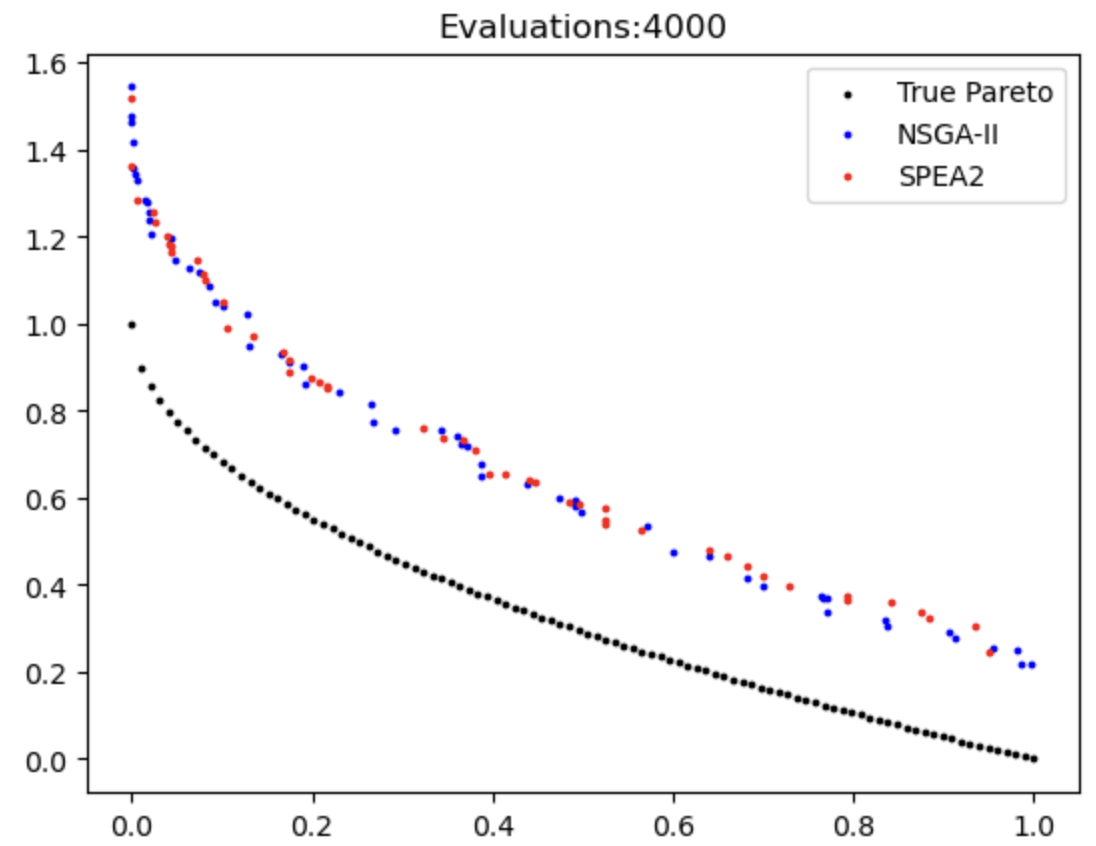
\includegraphics[width = 1.5in]{ZDT1_4e3.png}} &
\subfloat[ZDT1:8000]{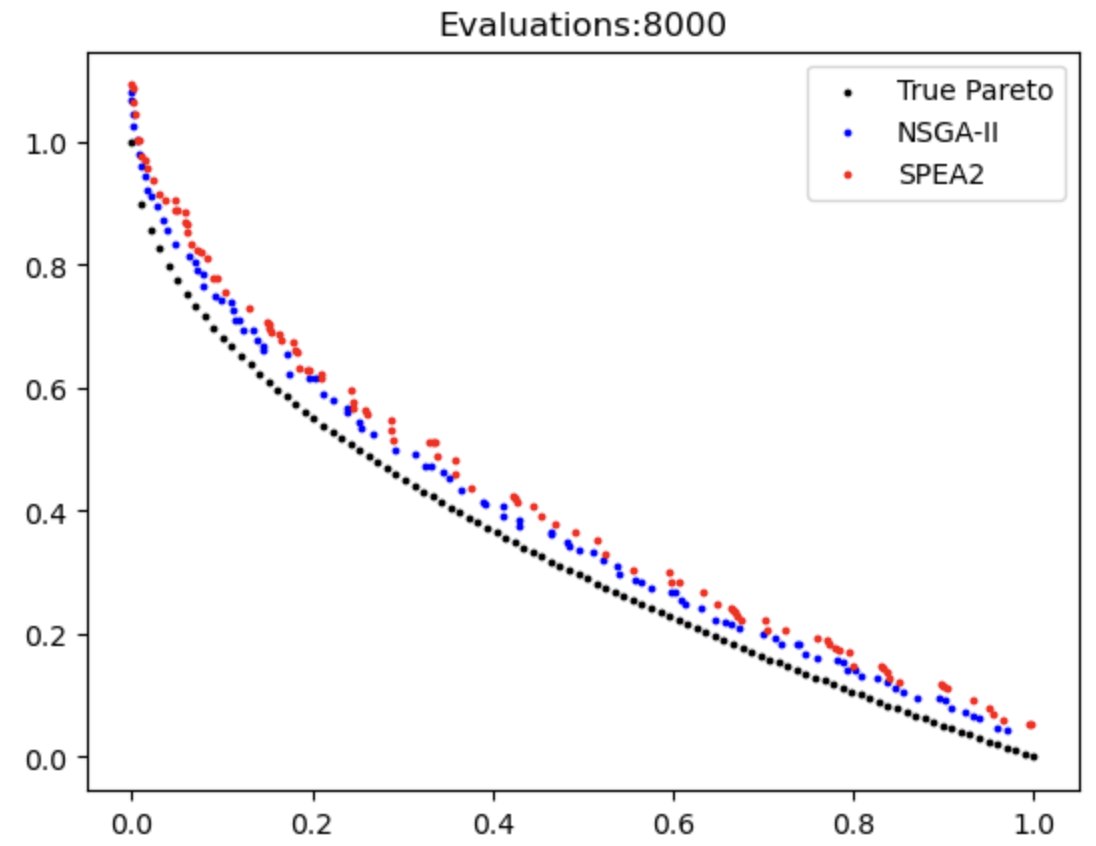
\includegraphics[width = 1.5in]{ZDT1_8e3.png}} &
\subfloat[ZDT1:12000]{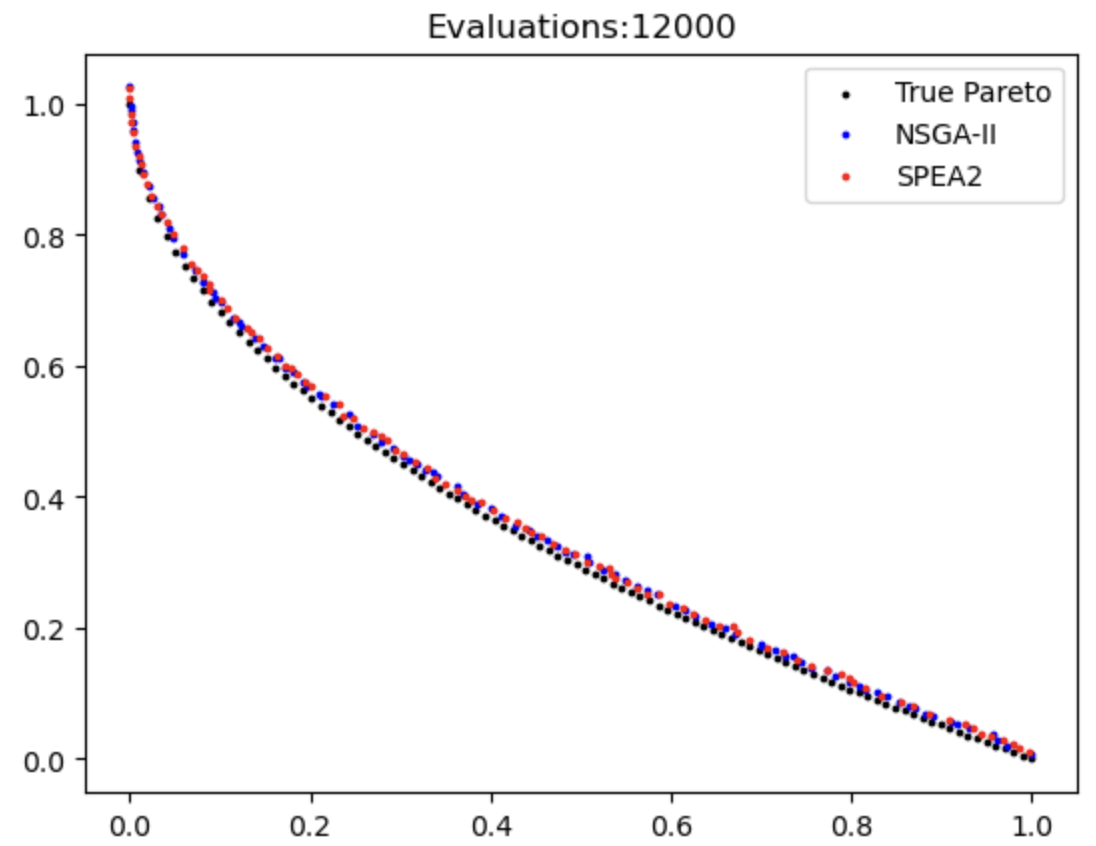
\includegraphics[width = 1.5in]{ZDT1_12e3.png}} &
\subfloat[ZDT1:16000]{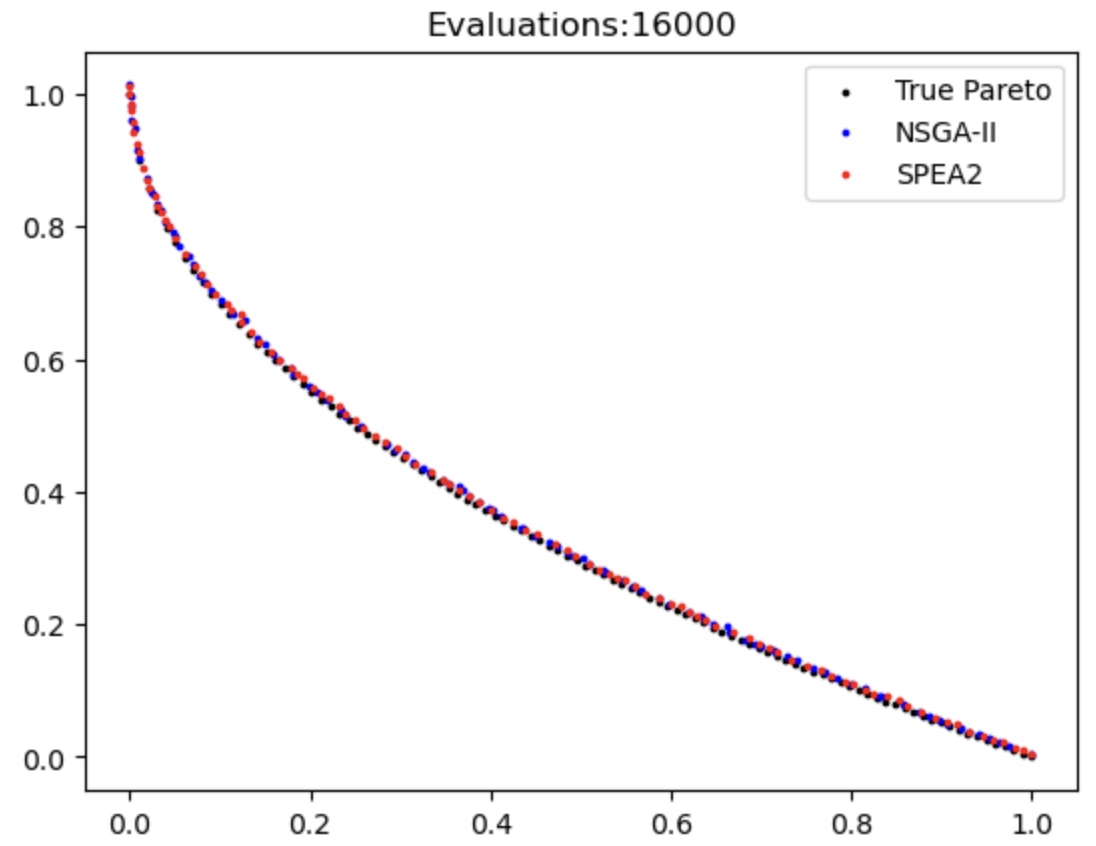
\includegraphics[width = 1.5in]{ZDT1_16e3.png}}\\
\subfloat[ZDT2:4000]{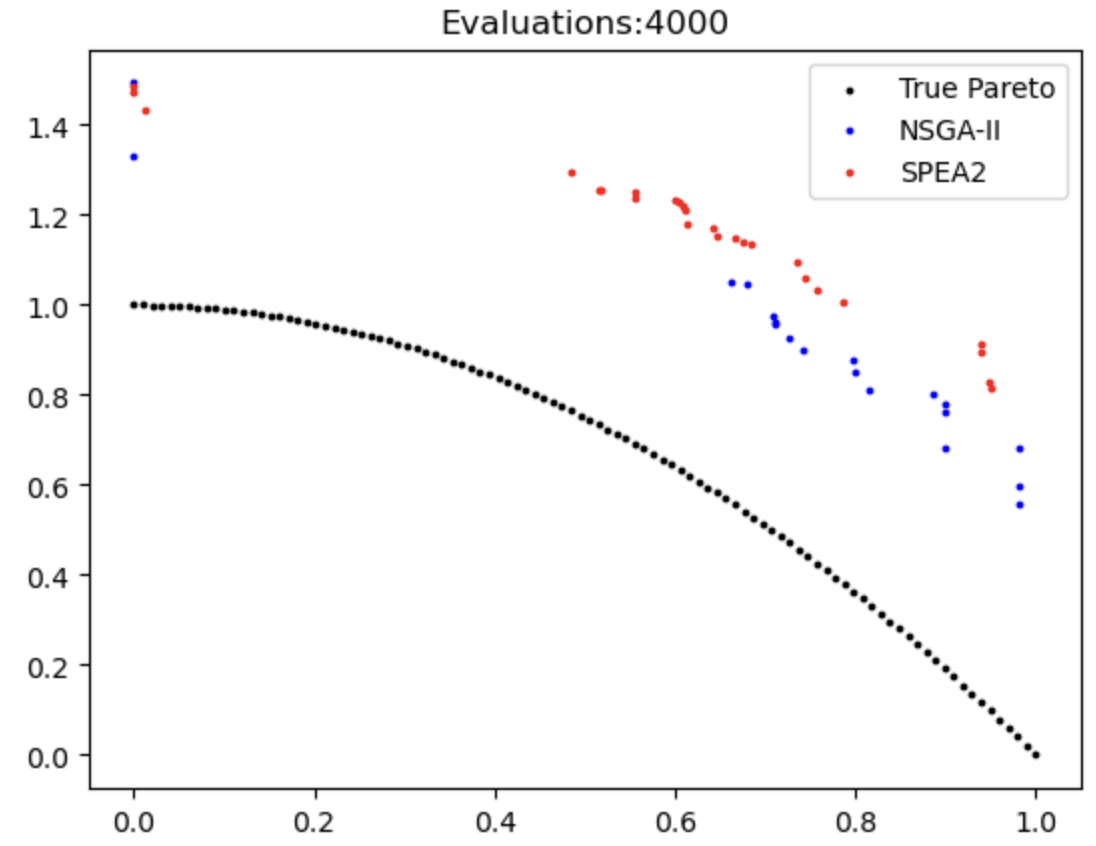
\includegraphics[width = 1.5in]{ZDT2_4e3.png}} &
\subfloat[ZDT2:8000]{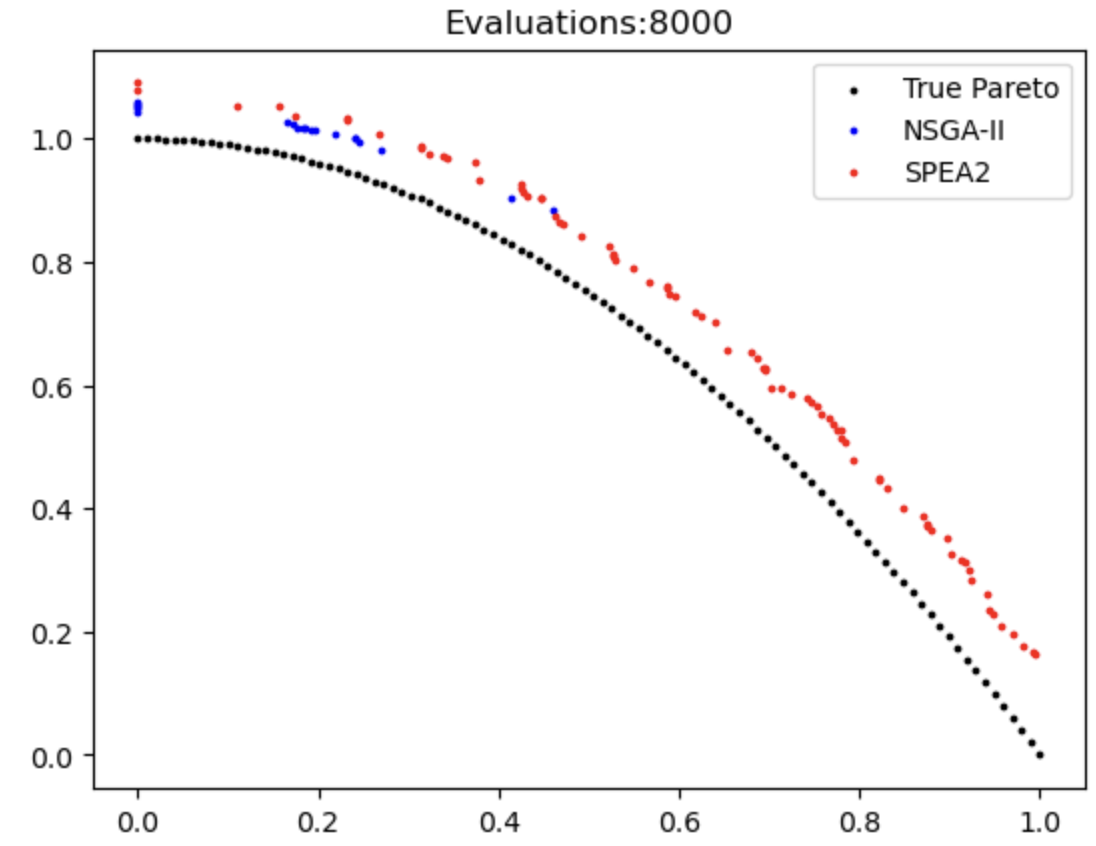
\includegraphics[width = 1.5in]{ZDT2_8e3.png}} &
\subfloat[ZDT2:12000]{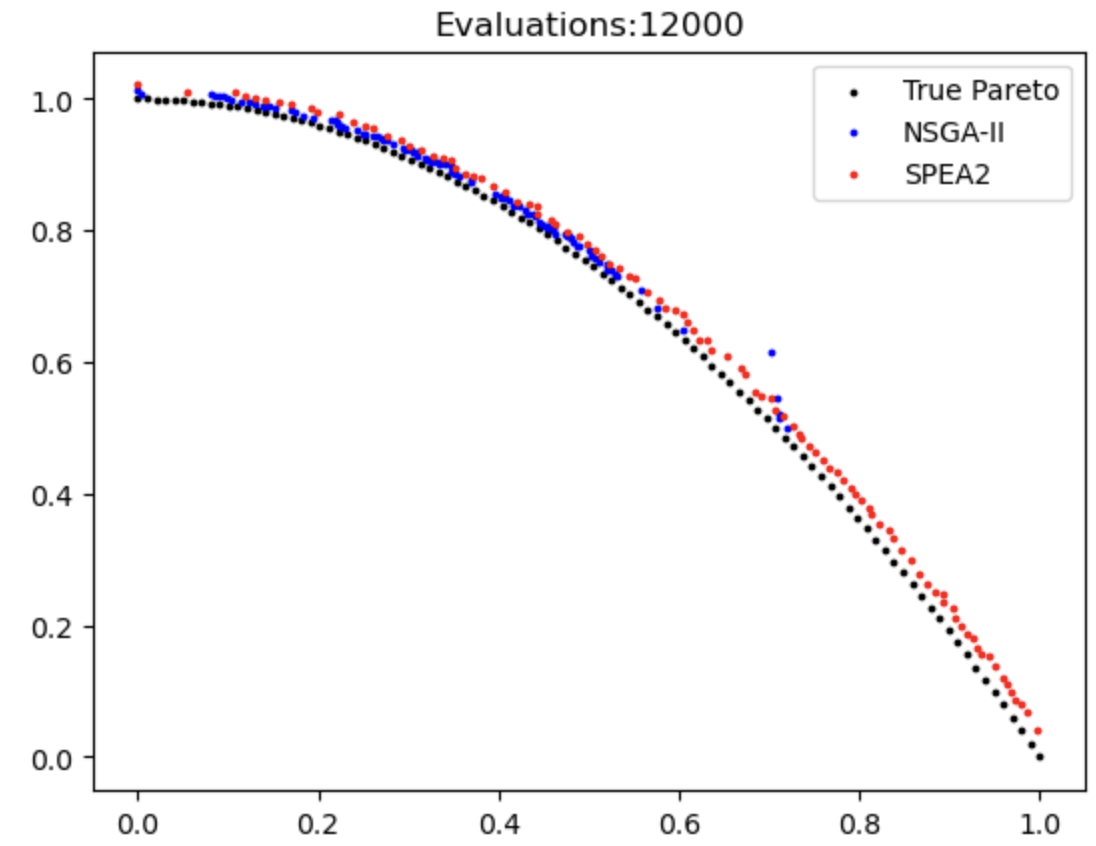
\includegraphics[width = 1.5in]{ZDT2_12e3.png}} &
\subfloat[ZDT2:16000]{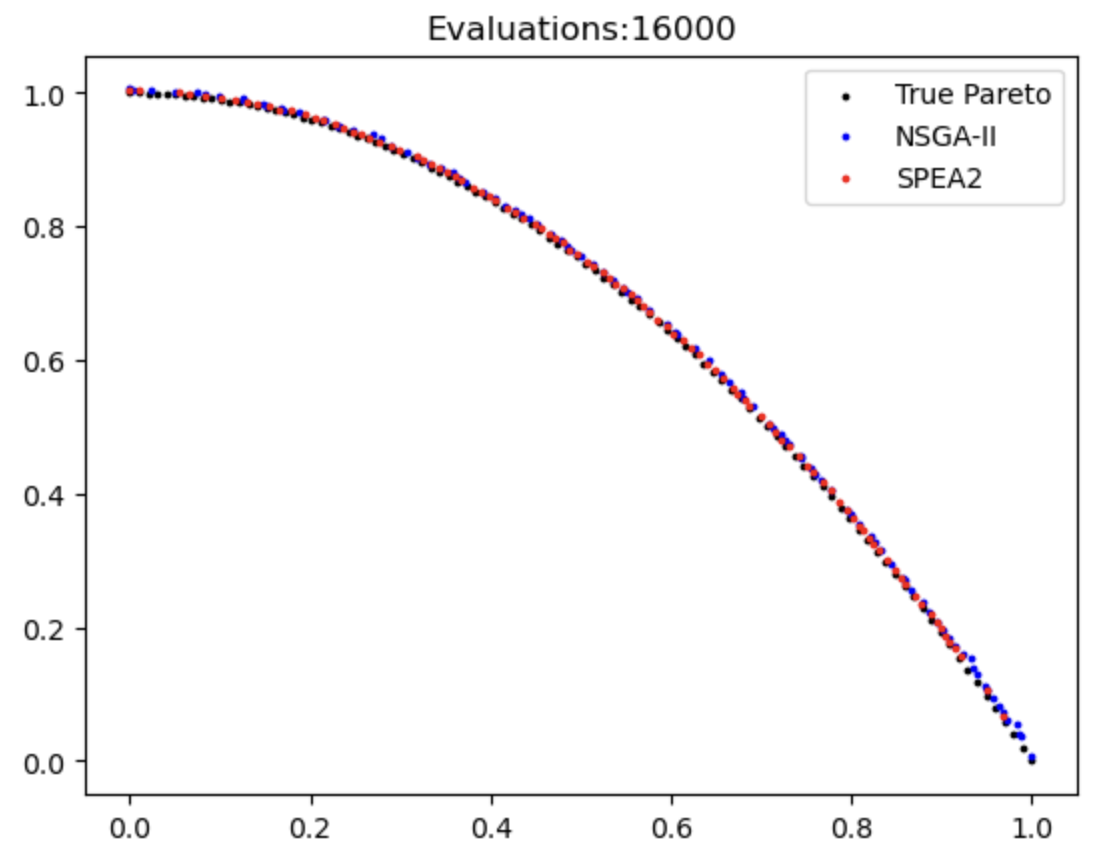
\includegraphics[width = 1.5in]{ZDT2_16e3.png}}\\
\subfloat[ZDT3:4000]{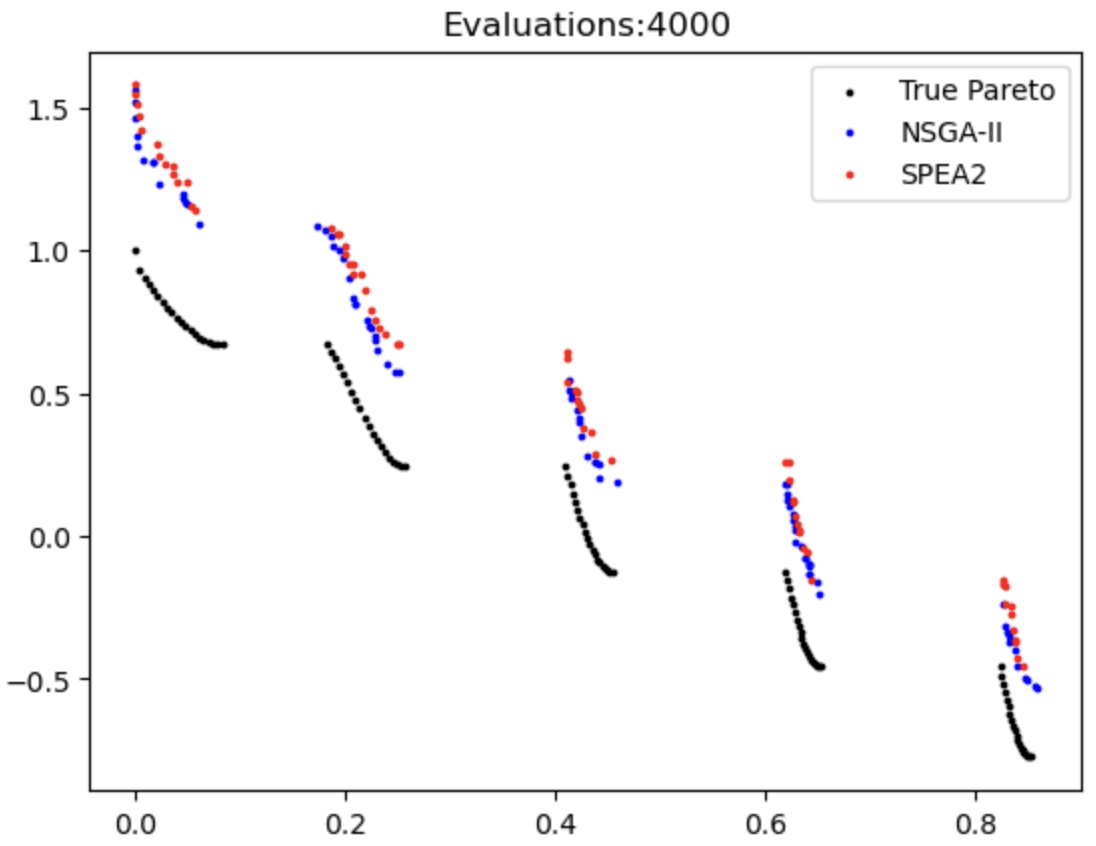
\includegraphics[width = 1.5in]{ZDT3_4e3.png}} &
\subfloat[ZDT3:8000]{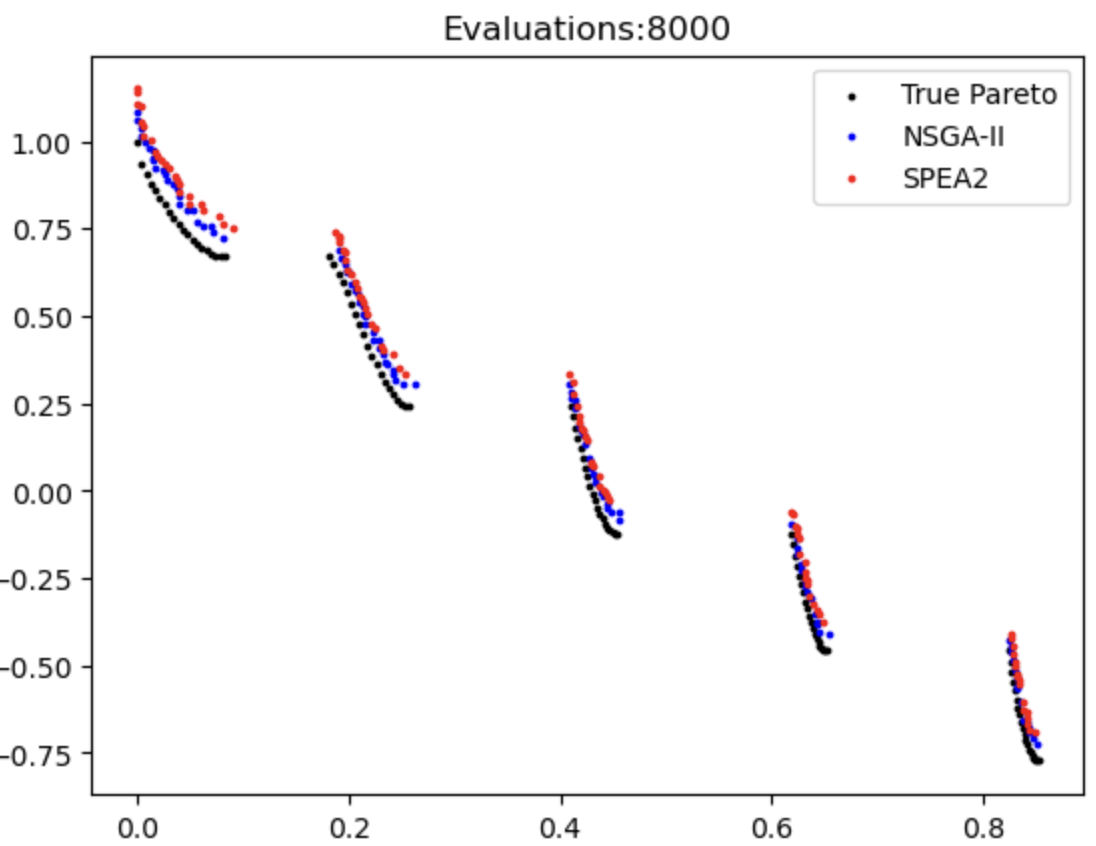
\includegraphics[width = 1.5in]{ZDT3_8e3.png}} &
\subfloat[ZDT3:12000]{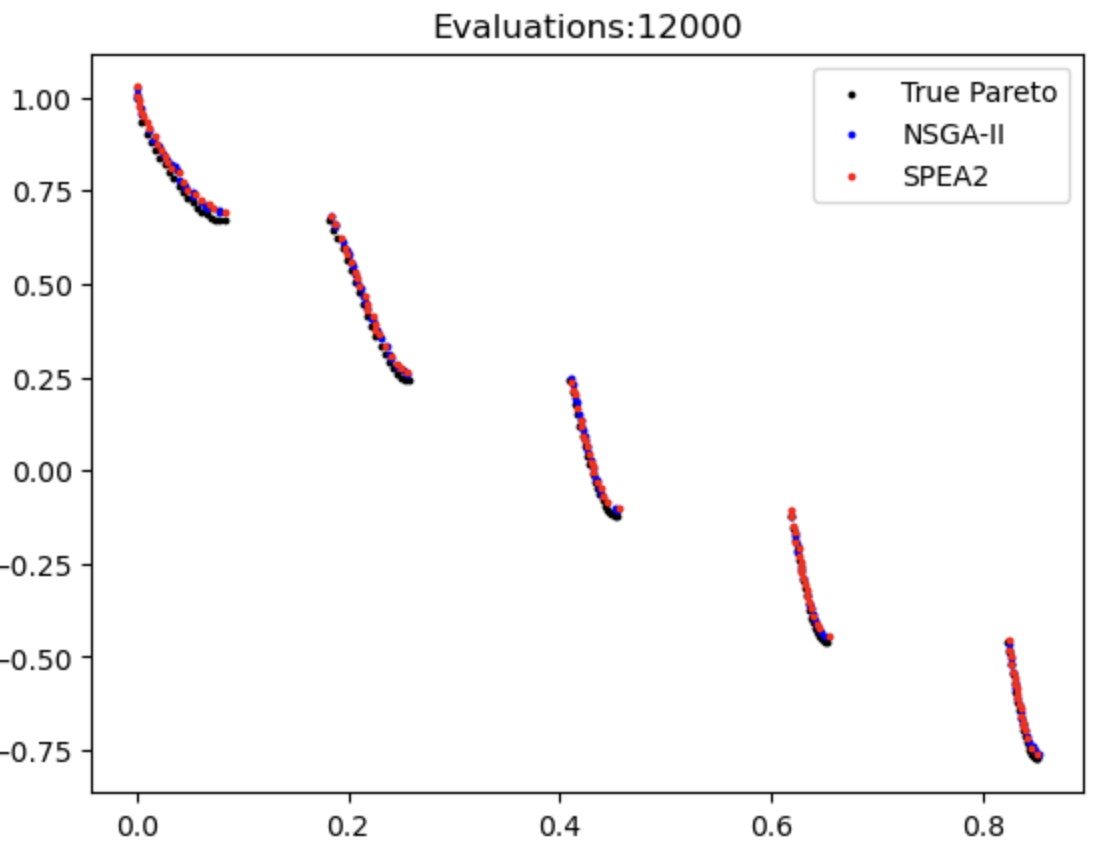
\includegraphics[width = 1.5in]{ZDT3_12e3.png}} &
\subfloat[ZDT3:16000]{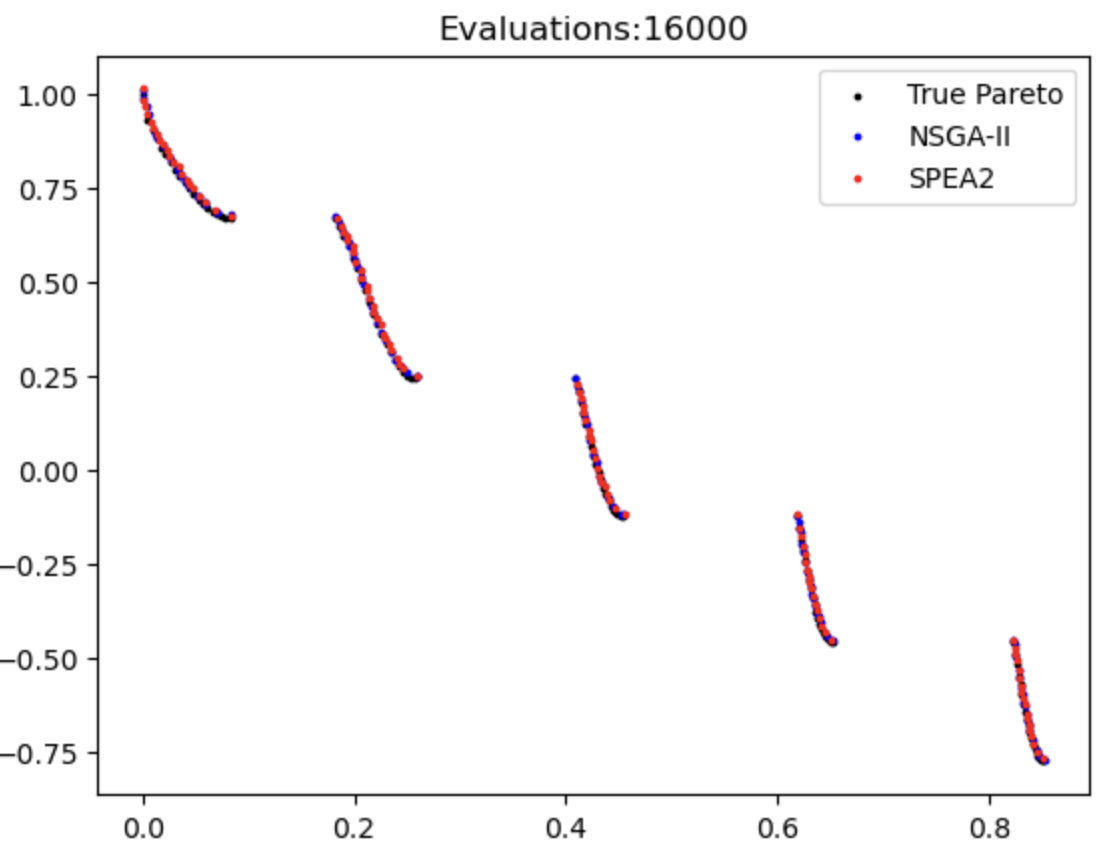
\includegraphics[width = 1.5in]{ZDT3_16e3.png}}\\
\subfloat[ZDT4:4000]{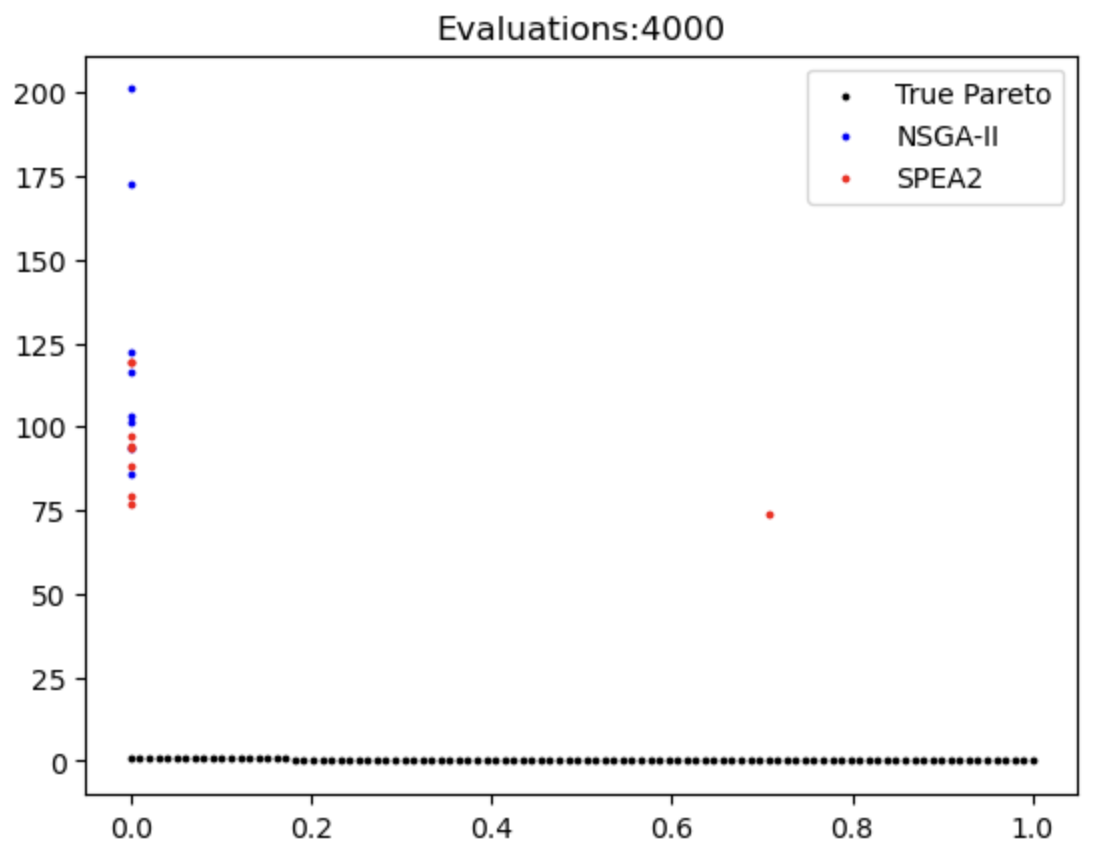
\includegraphics[width = 1.5in]{ZDT4_4e3.png}} &
\subfloat[ZDT4:28000]{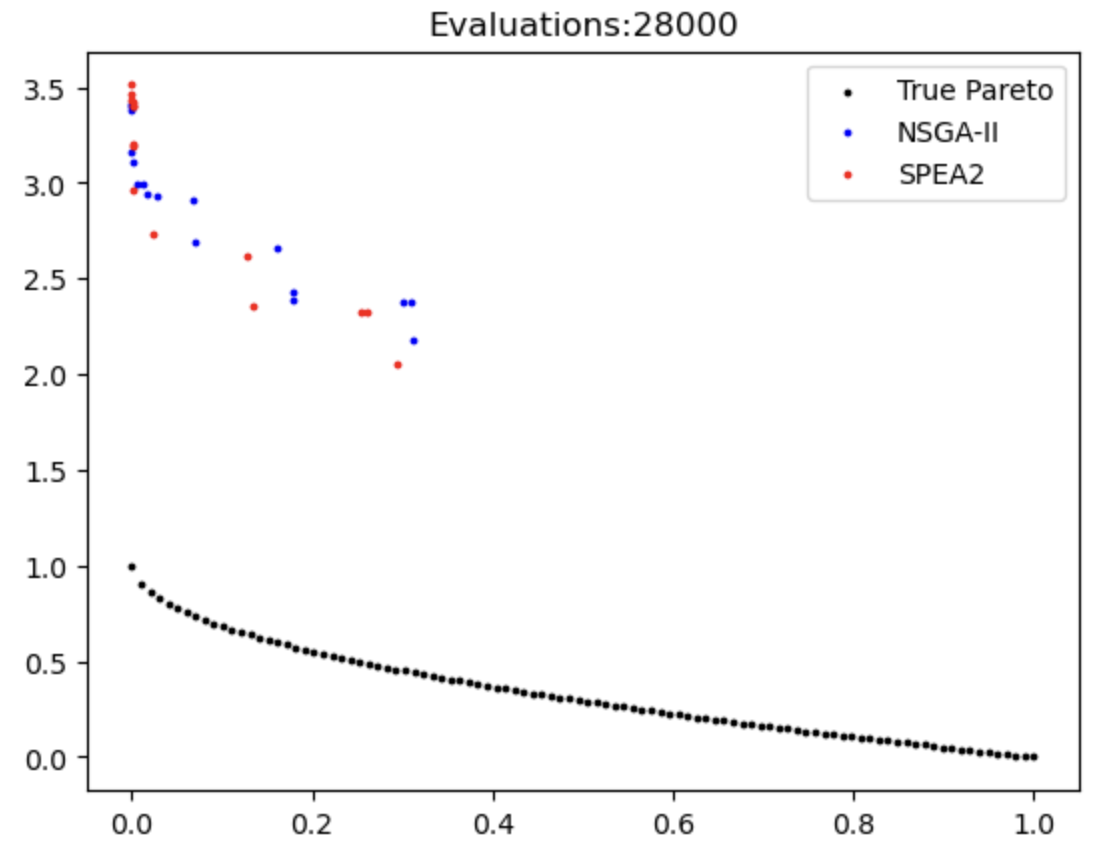
\includegraphics[width = 1.5in]{ZDT4_28e3.png}} &
\subfloat[ZDT4:54000]{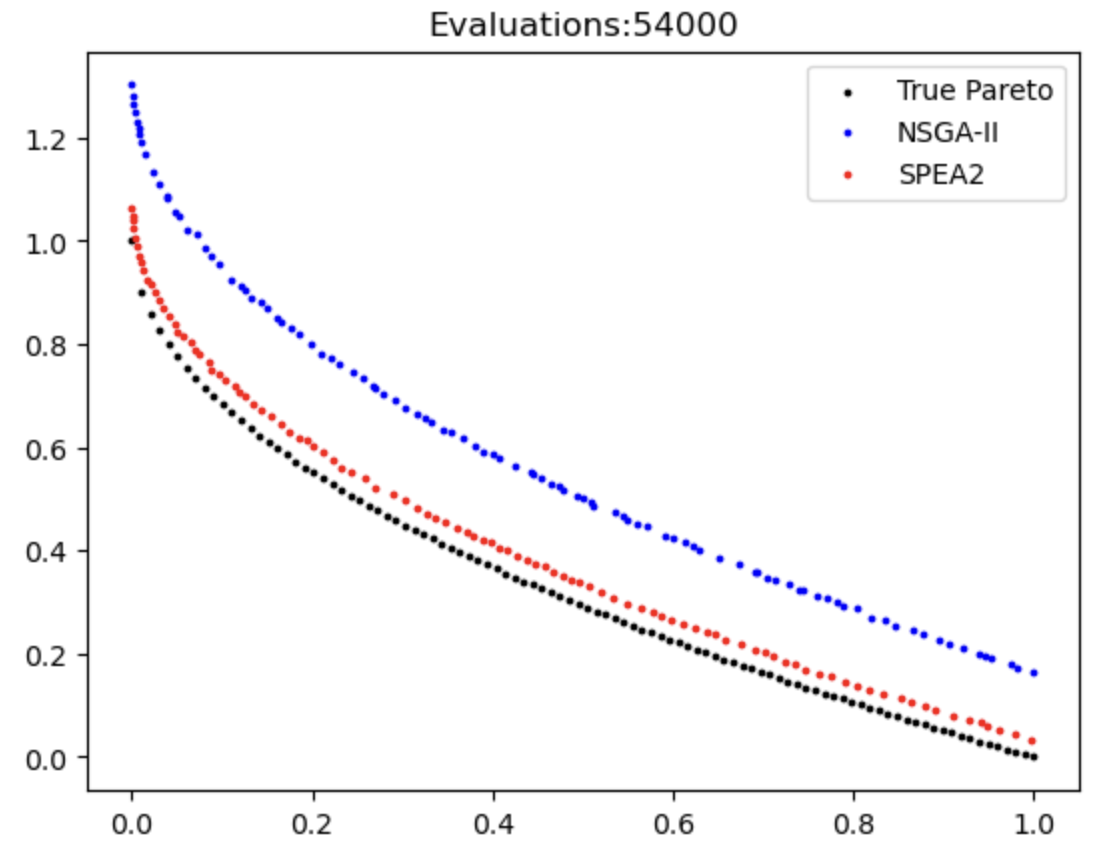
\includegraphics[width = 1.5in]{ZDT4_54e3.png}} &
\subfloat[ZDT4:72000]{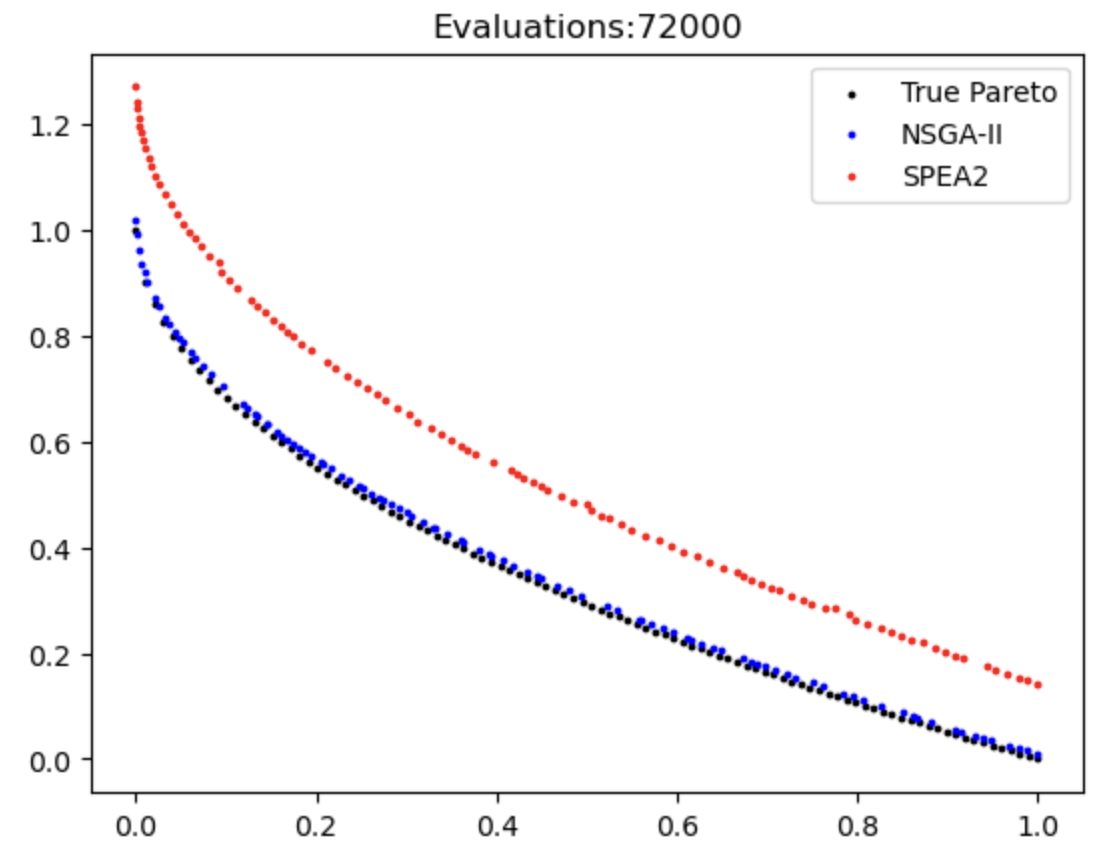
\includegraphics[width = 1.5in]{ZDT4_72e3.png}}\\
\subfloat[ZDT6:4000]{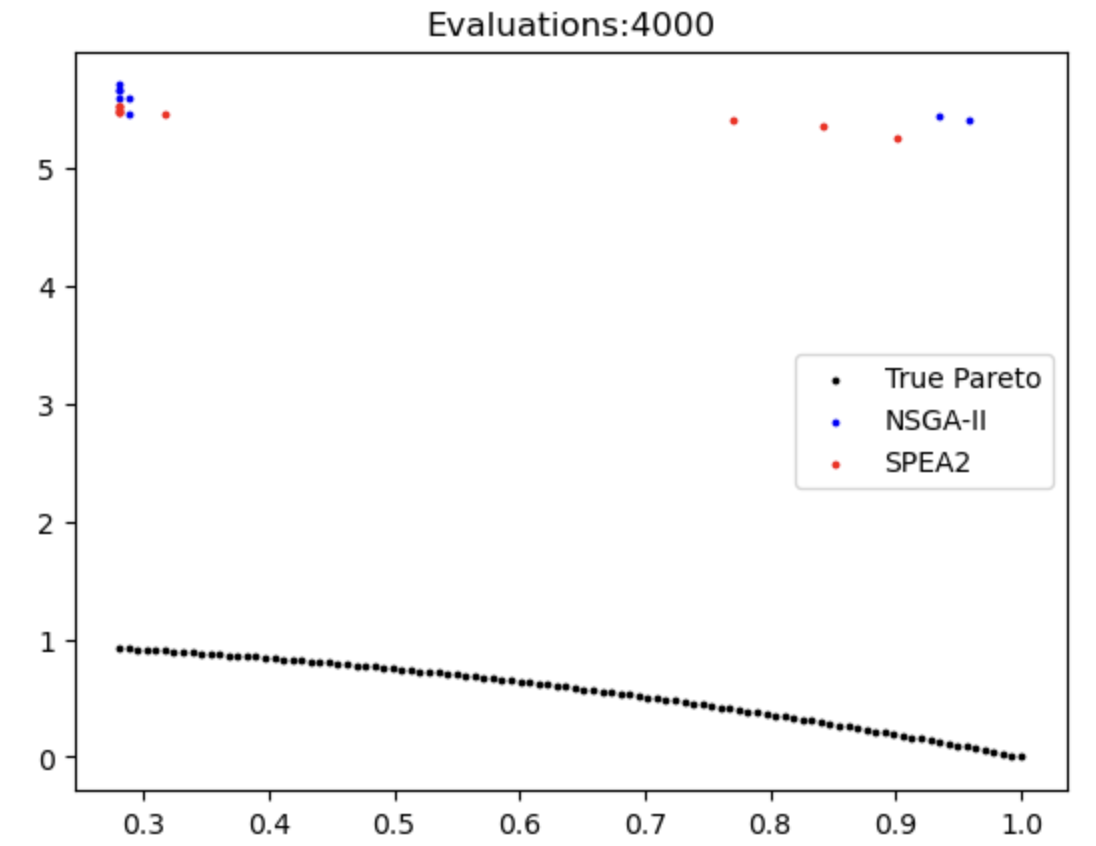
\includegraphics[width = 1.5in]{ZDT6_4e3.png}} &
\subfloat[ZDT6:28000]{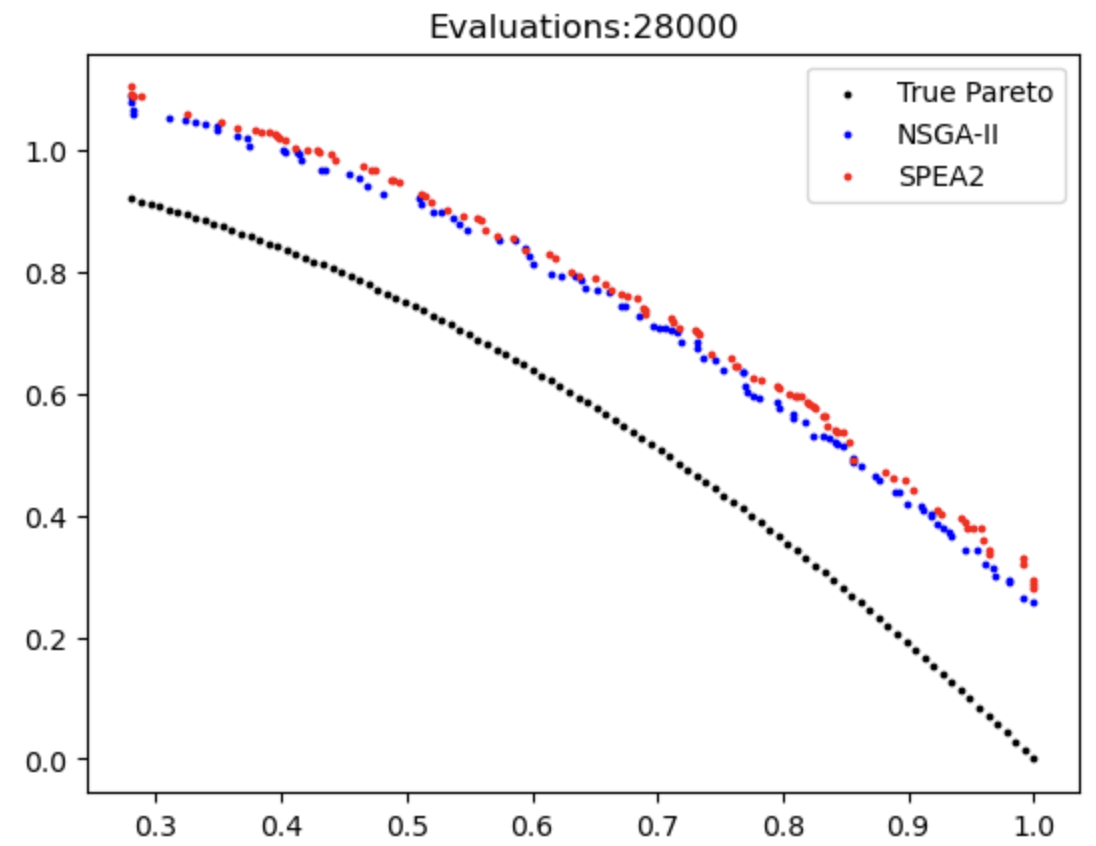
\includegraphics[width = 1.5in]{ZDT6_28e3.png}} &
\subfloat[ZDT6:54000]{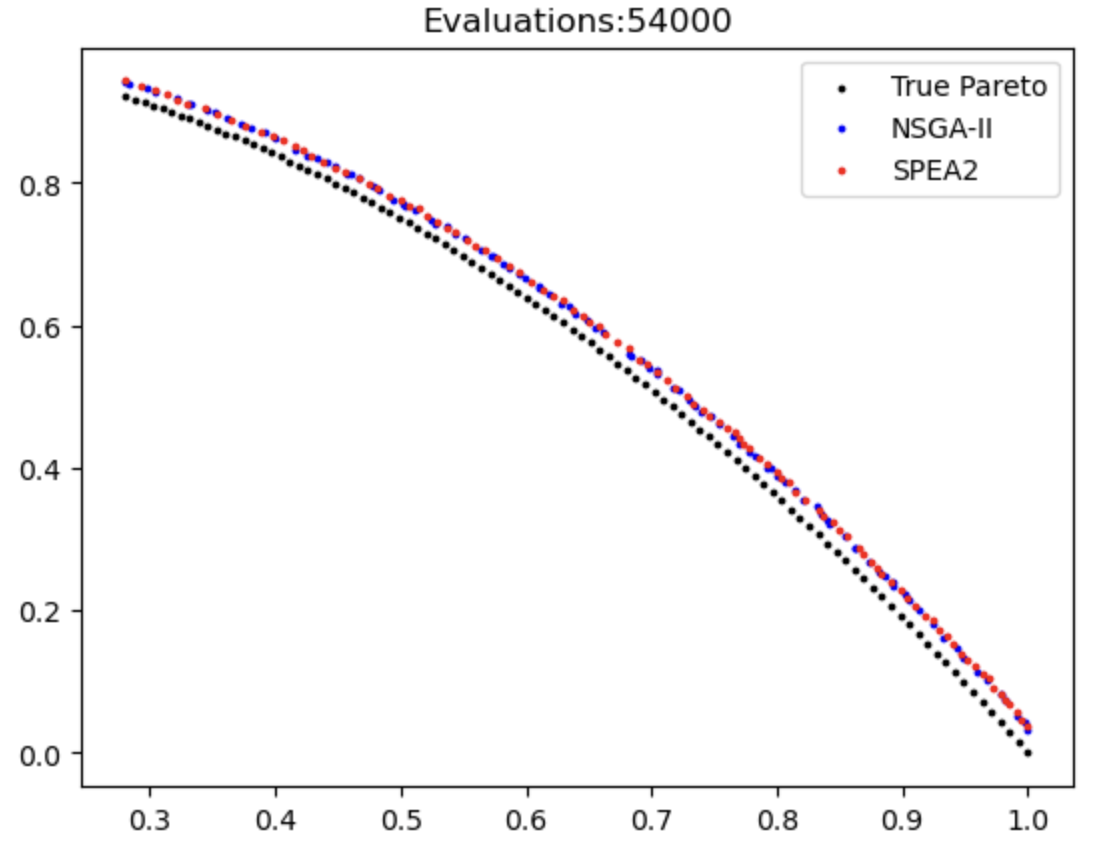
\includegraphics[width = 1.5in]{ZDT6_54e3.png}} &
\subfloat[ZDT6:72000]{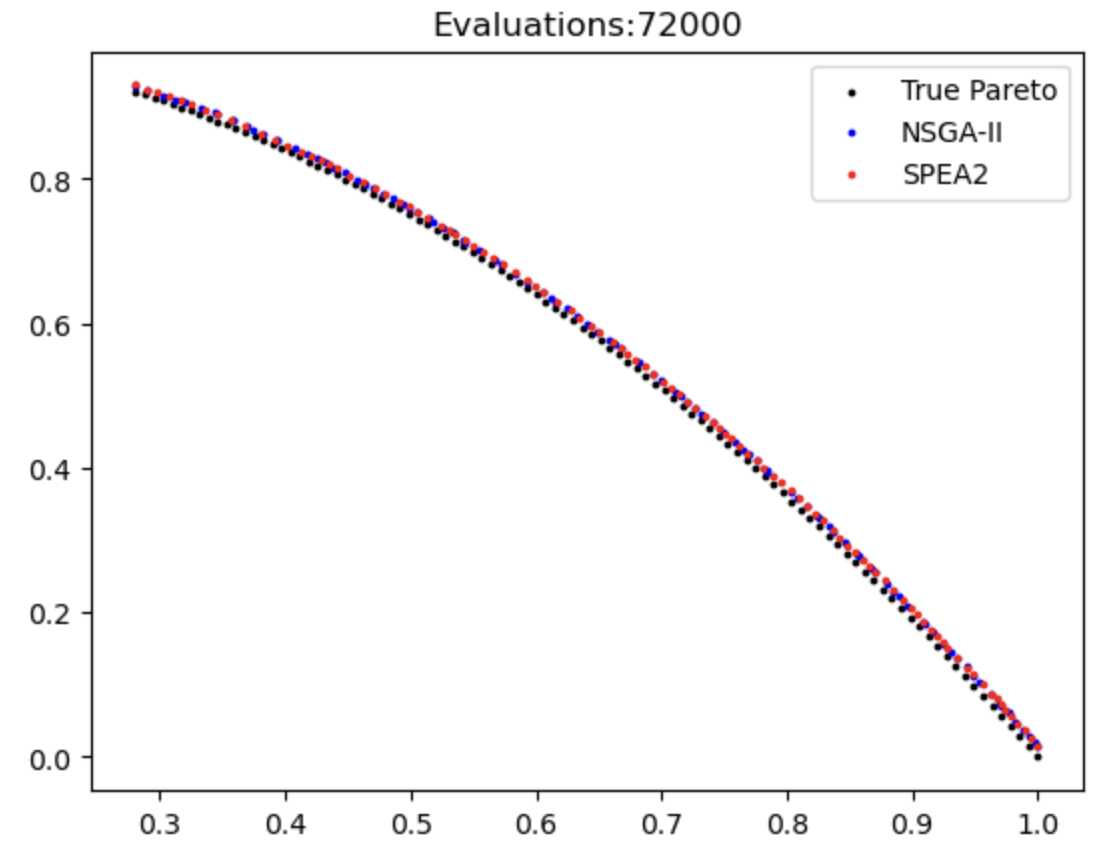
\includegraphics[width = 1.5in]{ZDT6_72e3.png}}
\end{tabular}
\caption{For the above simulations, the problem name and number of evaluations are given as graph titles. The \underline{\textcolor{blue}{blue}} points represent set of solutions for NSGA-II, and the \underline{\textcolor{red}{red}} points represent set of solutions for SPEA2, while the \underline{black} points represent the true Pareto front}
\end{figure*}
\begin{table*}
    \centering
    \begin{tabular}{|c|c|c|c|c|c|c|c|c|c|c|}
    \hline
         \multirow{2}{3em}{Problem} & \multirow{2}{4.5em}{Evaluations} & \multicolumn{2}{|c|}{IGD} & \multicolumn{2}{|c|}{$\Delta$-metric} & \multicolumn{3}{|c|}{Hypervolume Indicator} & \multicolumn{2}{|c|}{Number of solutions}\\
         \cline{3-11}
         & & NSGA-II & SPEA2 & NSGA-II & SPEA2 & NSGA-II & SPEA2 & True Pareto & NSGA-II & SPEA2\\
         \hline
         \multirow{4}{3em}{ZDT1} & 4000 & 0.171 & 0.1477 & 0.046 & 0.048 & 0.731 & 0.769 & 0.992 & 57 & 44 \\
         & 8000 & 0.028 & 0.025 & 0.029 & 0.023 & 0.674 & 0.677 & 0.714 & 100 & 100\\
         & 12000 & 0.009 & 0.008 & 0.05 & 0.045 & 0.663 & 0.664 & 0.674 & 100 & 100\\
         & 16000 & 0.006 & 0.006 & 0.006 & 0.006 & 0.67 & 0.67 & 0.675 & 100 & 100\\
         \hline
         \multirow{4}{3em}{ZDT2} & 4000 & 0.394 & 0.449 & 0.108 & 0.098 & 0.418 & 0.345 & 0.938 & 23 & 19\\
         & 8000 & 0.045 & 0.049 & 0.027 & 0.023 & 0.326 & 0.322 & 0.392 & 31 & 73 \\
         & 12000 & 0.088 & 0.014 & 0.02 & 0.022 & 0.125 & 0.125 & 0.137 & 54 & 100 \\
         & 16000 & 0.006 & 0.006 & 0.029 & 0.022 & 0.324 & 0.325 & 0.331 & 100 & 100\\
         \hline
         \multirow{4}{3em}{ZDT3} & 4000 & 0.16 & 0.176 & 0.058 & 0.056 & 0.964 & 0.939 & 1.28 & 44 & 74\\
         & 8000 & 0.02 & 0.033 & 0.056 & 0.068 & 0.809 & 0.784 & 0.853 & 100 & 100\\
         & 12000 & 0.009 & 0.007 & 0.036 & 0.041 & 0.788 & 0.795 & 0.807 & 100 & 100\\
         & 16000 & 0.005 & 0.005 & 0.037 & 0.035 & 0.776 & 0.777 & 0.782 & 100 & 100\\
         \hline
         \multirow{4}{3em}{ZDT4} & 4000 & 96.05 & 62.62 & 0.24 & 0.354 & 7.545 & 1.042 & 1.461 & 6 & 8\\
         & 28000 & 1.956 & 1.937 & 0.047 & 0.04 & 1.756 & 1.369 & 3.869 & 12 & 17\\
         & 54000 & 0.0813 & 0.095 & 0.123 & 0.0227 & 0.51 & 0.527 & 0.619 & 100 & 100\\
         & 72000 & 0.01 & 0.135 & 0.039 & 0.023 & 0.918 & 0.745 & 0.93 & 100 & 100\\
         \hline
         \multirow{4}{3em}{ZDT6} & 4000 & 4.155 & 4.399 & 0.122 & 0.25 & 0.13 & 0.157 & 0.33 & 11 & 6\\
         & 28000 & 0.138 & 0.151 & 0.0209 & 0.0217 & 0.235 & 0.222 & 0.386 & 100 & 100\\
         & 54000 & 0.017 & 0.018 & 0.0208 & 0.0207 & 0.2613 & 0.2606 & 0.2816 & 100 & 100\\
         & 72000 & 0.006 & 0.007 & 0.021 & 0.021 & 0.263 & 0.263 & 0.27 & 100 & 100\\
         \hline
    \end{tabular}
    \caption{Results from running simulations for different number of evaluations (run time)}
\end{table*}
\subsection{ZDT1}
For the run times $\{4000, 8000, 12000, 16000\}$, it can be observed that whilst both MOEAs do not represent accurate set of solutions for the first one, NSGA-II outperforms SPEA2 for other run times. In addition to this, the IGD- and $\Delta$-metric consistently reduces down to $\approx 0.00$ when evaluations increase, whilst the Hypervolume indicator reaches the measure close to the true Pareto front. Other than these, there were no extreme insights and the metrics demonstrated magnitudes which were well expected.
\subsection{ZDT2}
For the same run times used as for ZDT1, the first one starts off with the worst performance, where both MOEAs generated scattered randomly, thus the high $\Delta$ value. However, for the next two run times, ${8000, 12000}$, the number of solutions generated by NSGA-II (31) are much less than SPEA2 (73); Despite of this, the $\Delta$-metric is not that drastic for NSGA-II when compared to SPEA2 - this potentially could be a discrepancy on the application of this metric towards this type of a problem. For this problem, SPEA2 seems to outperform NSGA-II.
\subsection{ZDT3}
For the same run times used as for ZDT1, for the first run, it seems that the number of solutions generated by NSGA-II is markedly less than SPEA2. Despite of this, the $\Delta$-metric is almost identical for both MOEAs. Given the well-spread nature of this problem, the diversity of solutions for NSGA-II is questionable, considering the number of solutions generated. This confirms that $\Delta$-metric may not seem that meaningful to interpret results, and one has to consider other metrics such as visual inspection and number of solutions generated. On the other hand, the two metrics, IGD and Hypervolume, seem to be helpful in interpreting the effectiveness of MOEAs towards this problem - the first run presenting worst results, and consistently improves with higher run time.
\subsection{ZDT4}
The run times considered are $\{4000, 28000, 54000, 72000\}$ for the ZDT4 problem. The first run generates very few solutions, not remotely close to the true Pareto front. For the second run, the solutions are scattered, yet far from the true Pareto front - and therefore, IGD is significantly high. Surprisingly, the $\Delta$-metric is 0.04, which theoretically means that the solutions generated are good. However, considering figure 1(n), such solutions cannot be said to be well-spread and diverse. Again, it could be said that $\Delta$-metric is not meaningful in this problem. On hypervolume indicator, NSGA-II is closer to true Pareto front, and as observed from visual representation, NSGA-II significantly outperforms SPEA2. Additionally, the SPEA2 seems to be presenting the same pareto front between 54000 to 72000, reaching its optimum convergence in finding solutions, irrespective of any run time beyond 54000.
\subsection{ZDT6}
The run times considered are the same as ZDT4. As expected, both MOEAs perform poorly for the first run. For the other three runs, the results consistently improve, and these are apparent with all three PIs, IGD, $\Delta$-metric, and hypervolume indicator. For this problem, NSGA-II starts off with a better performance (as observed in Figure 1(r)), but for higher run times, both MOEAs perform equivalently well.

\section{Discussion and future work}
It is apparent that IGD and Hypervolume indicator requires the true Pareto front to be known, as this is used as a reference to compare efficiency of MOEAs. The diversity metric, $\Delta$-metric, is the only exception, where diversity of solutions could be assessed without the need for having any information on the true Pareto front. However, it comes with limitations. Yan \textit{et al.} \cite{yan2007} rightly point this discrepancy of using $\Delta$-metric towards assessing diversity of solutions, which was also recognised when performing analysis. $\Delta$-metric did not seem effective in problems ZDT2, ZDT3, and ZDT4, where the magnitude represented promising result, however, this was not the case when visual representations were considered. One of the reasons of this inaccuracy could be due to the fact that only extreme points and the distances within them are considered (as per the formula), with no reference to the true Pareto front, the solutions between extreme points might be well-spread and uniform, however, they would not represent diverse solutions in context to the true Pareto front. Cai \textit{et al.} \cite{cai2018} present a diversity metric that they claim is more efficient than the $\Delta$-metric. They employ a \textit{coverage vector}, where different angles are drawn from the origin $(0.00, ..., 0.00)_{n}$, where $n$ is the number of dimensions, which is then incorporated to the $DIR$-metric. The $DIR$-metric accounts for both uniformity and coverage of solutions. A similar PI that considers both distribution and convergence is the use of attainment surfaces, where lines from different angles are drawn from the origin, and the distances between multiple Pareto fronts are compared in ranking different MOEAs \cite{bui2005}. Other convergence- and divergence-based PIs might also be effective in this case. \\
\begin{figure}
\centering
    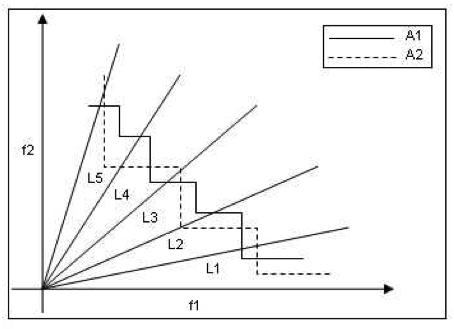
\includegraphics[width=70mm]{Screenshot 2023-07-21 at 02.11.30.png}
    \caption{Use of attainment surfaces: \textit{A1} and \textit{A2} are two Pareto fronts. Multiple surfaces (beyond two-dimensions)/ lines (for two-dimensions) are drawn from the origin $(0.00,...,0.00)_{n}$ and distances of the two fronts are measured \cite{bui2005}}
    \label{fig:enter-label}
\end{figure}
Whilst IGD and hypervolume indicator seem meaningful in presenting results across ZDT problems considered, it would be interesting to analyse whether this accuracy stays true for higher dimensional problems, such as DTLZ. This could potentially be a future work to develop on this study further. \\
Additionally, it is observed that for ZDT2 with run times 8000 and 12000, the solutions for NSGA-II are not that diverse and the number of solutions is much less than expected, whilst SPEA2 performs as expected. Although this has just occurred for 2 of 20 simulations performed, which might show that such situations are rare, this is unusual behaviour for NSGA-II as the algorithm explicitly accounts for diversity preservation (see section \ref{Background_nsgaii}). By running further simulations for run times with an increment of 1000 from the range (4000, 12000), it might be more apparent to see whether this diversity preservation issues is demonstrated for all those simulations. 
\bibliographystyle{unsrt}
\bibliography{references.bib} 

\vfill\vfill\vfill\vfill
\onecolumn
\appendix
\section*{APPENDIX}
\subsection*{Code}
\begin{verbatim}
############################################################
This code pertains for both 2D and 3D problems. As 3D
problems took a very long time, these were not used towards
the report. They were experimented upon, nevertheless.
############################################################

# Pymoo for visualising True Pareto
from pymoo.problems import get_problem
from pymoo.util.ref_dirs import get_reference_directions

# jMetalPy for importing MOEAs
from jMetalPy.jmetal.algorithm.multiobjective.nsgaii import NSGAII
from jMetalPy.jmetal.algorithm.multiobjective.spea2 import SPEA2

# jMetalPy operators and utilities libraries for performing MOEA analysis
from jMetalPy.jmetal.operator import SBXCrossover, PolynomialMutation
from jMetalPy.jmetal.problem.multiobjective.zdt import ZDT1, ZDT2, ZDT3, ZDT4, ZDT6
from jMetalPy.jmetal.problem.multiobjective.dtlz import DTLZ1, DTLZ2, DTLZ3, DTLZ4, DTLZ5, DTLZ6, DTLZ7
from jMetalPy.jmetal.util.termination_criterion import StoppingByEvaluations
from jMetalPy.jmetal.util.solution import get_non_dominated_solutions

# NumPy and Matplotlib for plotting
import matplotlib.pyplot as plt
import numpy as np

# SciPy and Pymoo for Performance Indicators
from scipy.spatial.distance import cdist
from pymoo.indicators.igd import IGD
from pymoo.indicators.hv import HV

# Importing a specific problem for analysis -- Replace 'zdt4' and ZDT4 to your choice
p = get_problem('zdt4')
#ref_dirs = get_reference_directions('das-dennis', n_dim=3, n_partitions=13)  ## Only used for 3D problems
pareto = p.pareto_front()
problem = ZDT4(number_of_variables=30)

# MOEAs to use towards the problem
max_evaluations = 72e3    # Run time
algorithm1 = NSGAII(
    problem=problem,
    population_size=100,
    offspring_population_size=100,
    mutation=PolynomialMutation(probability= 1.0/30.0, distribution_index=20),
    crossover=SBXCrossover(probability=1.0, distribution_index=20),
    termination_criterion=StoppingByEvaluations(max_evaluations)
)
algorithm2 = SPEA2(
    problem=problem,
    population_size=100,
    offspring_population_size=100,
    mutation=PolynomialMutation(probability= 1.0/30.0, distribution_index=20),
    crossover=SBXCrossover(probability=1.0, distribution_index=20),
    termination_criterion=StoppingByEvaluations(max_evaluations)
)
algorithm1.run()
algorithm2.run()
solutions1 = algorithm1.get_result()
solutions2 = algorithm2.get_result()

# Retrieve Pareto fronts for NSGA-II and SPEA2
front1 = get_non_dominated_solutions(solutions1)
front2 = get_non_dominated_solutions(solutions2)
nsgaii_front = Plot.get_points(front1)
spea2_front = Plot.get_points(front2)

# Print IGD measures for both MOEA
ind = IGD(pareto)
nsgaii_front = np.array(nsgaii_front)
spea2_front = np.array(spea2_front)
print("IGD [NSGA-II]:", ind(nsgaii_front))
print("IGD [SPEA2]:", ind(spea2_front))

# Print delta-metric for both MOEA
def delta_metric(algo_front, true_front):
    n = len(algo_front)
    distances = cdist(algo_front, true_front, metric='euclidean')
    closest_distances = np.min(distances, axis=1)
    df = np.min(closest_distances)
    dl = np.max(closest_distances)
    d_avg = np.mean(closest_distances)
    delta = (df + dl + np.sum(closest_distances - d_avg)) / (df + dl + (n - 1) * d_avg)
    return delta

nsgaii_front = np.array(nsgaii_front)
spea2_front = np.array(spea2_front)
delta1 = delta_metric(nsgaii_front, pareto)
delta2 = delta_metric(spea2_front, pareto)
print('Delta [NSGA-II]:', delta1)
print('Delta [SPEA2]:', delta2)

# Print Hypervolume metric for both MOEA
nsgaii_front = np.array(nsgaii_front)
spea2_front = np.array(spea2_front)

if delta1 > delta2:
    ref_point = np.max(spea2_front, axis=0)
else:
    ref_point = np.max(nsgaii_front, axis=0)

ind = HV(ref_point=ref_point)

print('HV [NSGA-II]:', ind(nsgaii_front))
print('HV [SPEA2]:', ind(spea2_front))
print('True_HV', ind(np.array(pareto)))

# Plot MOEA solutions with reference to true Pareto
if len(nsgaii_front[0]) == 3:
    fig = plt.figure(figsize = (10, 7))
    ax = plt.axes(projection ="3d")
    ax.scatter3D(*zip(*pareto), c='k', s=5, label='True Pareto')
    ax.scatter3D(*zip(*nsgaii_front), c='b', s=5, label='NSGA-II')
    ax.scatter3D(*zip(*spea2_front), c='r', s=5, label='SPEA2')
elif len(nsgaii_front[0]) == 2:
    plt.scatter(*zip(*pareto), c='k', s=3, label='True Pareto')
    plt.scatter(*zip(*nsgaii_front), c='b', s=3, label='NSGA-II')
    plt.scatter(*zip(*spea2_front), c='r', s=3, label='SPEA2')

plt.title(f'Evaluations:%d' %max_evaluations)
plt.legend()
plt.show()
\end{verbatim}

\end{document}
